\chapter{牵引变电所主接线分析}
\section{开闭所主接线分析}
此处选取北宅站开闭所进行主接线分析,图\ref{海洋大学开闭所主接线图}为海洋大学开闭所主接线图。
\begin{figure}[h]
	\centering
	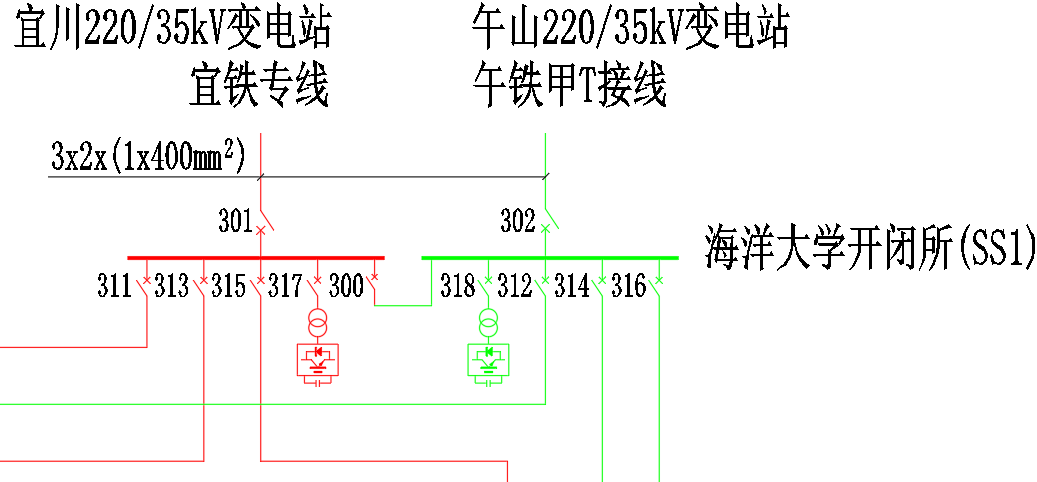
\includegraphics[width=0.5\textwidth]{海洋大学开闭所主接线图.png}
	\caption{海洋大学开闭所主接线图}
	\label{海洋大学开闭所主接线图}
\end{figure}
\subsection{接线方式}
北宅站开闭所$AC35kV$系统采用单母线接线方式,设有母线分段断路器;开闭所的两个$AC35kV$进线电源分别由上级城市电网变电站的两段不同的$AC35kV$母线,每段母线设置四回$AC35kV$馈线,其中三条回线为下级各变电所提供$35kV$电源,一条回线连接动态无功补偿装置(SVG);每段母线设置一套动态无功补偿装置(SVG),通过$AC35kV$断路器接到母线上。
\subsection{运行方式}
在正常运行情况下,存在两段母线并行运行,而$AC35kV$母线分段开关处于分闸状态。这两路进线电源各自为其供电范围内的变电所提供电力,承担其范围内的所有牵引负荷和动力照明负荷。


如果其中一路$35kV$进线电源发生停电情况,那么$AC35kV$母线分段开关将被自动或手动闭合,此时另一路$AC35kV$进线电源将为其供电范围内的变电所提供电力,同时承担其范围内的全部牵引负荷以及动力照明的一级和二级负荷。


但如果本开闭所的两路$AC35kV$进线电源均失电,且土寨河主变电所未建成,而中压环网确认无故障,另一开闭所的两个$AC35kV$电源仍处于正常状态,那么会采取以下措施:首先,切除全线的三级负荷,然后闭合位于蓝色硅谷站牵引降压混合变电所内的$AC35kV$应急联络开关。这将导致皋虞开闭所为全线提供应急支援供电,同时承担全线动力照明的一级和二级负荷以及部分牵引负荷。


如果土寨河主变电所已建成,当本开闭所退出运行时,将闭合位于北九水站降压所内的$AC35kV$应急联络开关,以便由土寨河主变电所提供应急支援供电。这种应急供电情况旨在确保牵引系统在突发情况下继续可靠运行。

\section{牵引/降压所主接线分析}
依照供电系统设计图资料,选取图\ref{浦鳌区间所牵引-降压主接线图}浦鳌区间所牵引-降压变电所为例进行分析。
\begin{figure}[h]
	\centering
	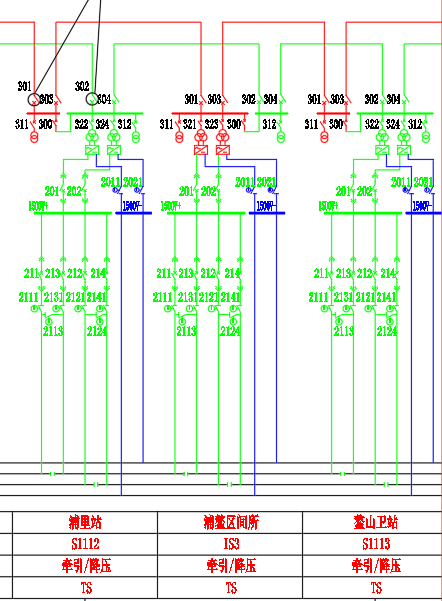
\includegraphics[width=0.6\textwidth]{浦鳌区间所牵引-降压主接线图.png}
	\caption{浦鳌区间所牵引-降压主接线图}
	\label{浦鳌区间所牵引-降压主接线图}
\end{figure}
\subsection{接线方式}
在$AC35kV$中压侧,采用分段单母线接线,并设置母线分段断路器。变电所的$1\#$进线电源引自上一站的变电所的$Ⅰ$段母线,而$2\#$进线电源则引自上一站的$Ⅱ$段母线。变电所配置了两台配电变压器,它们分别接在两段$AC35kV$母线上。此外,还设置了两套牵引套整流机组,它们都接在$AC35kV$的$Ⅰ$段或$Ⅱ$段母线上。这两套牵引整流机组并联运行,形成等效的24脉波整流。


至于$DC1500V$的牵引直流侧,采用了单母线接线。整流器的正极通过手车式直流快速断路器接到正母线上,而负极则通过电动隔离开关连接到直流负母线上。$DC1500V$系统设有4回出线,每一回通过手车式直流快速断路器连接到上行和下行电动上网隔离开关。牵引网的回流电缆直接与负极柜和上行、下行的走行轨连接。


对于车辆段的牵引变电所的$DC1500V$系统,配置了6回出线,每一回同样通过手车式直流快速断路器连接到电动上网隔离开关。牵引网的回流电缆也直接与负极柜以及车辆段内各供电分区的走行轨连接。

\subsection{运行方式}
在正常运行情况下,中压侧有两段母线并行运行,而$AC35kV$母线分段开关处于分闸状态。两路进线电源分别为各自供电范围内的全部牵引负荷和动力照明负荷提供电源。当其中一路$35kV$进线电源失电时,会闭合$35kV$母线分段开关,通过分段断路器,由一路$35kV$进线电源为该变电所供电范围内的全部牵引负荷和动力照明的一、二级负荷提供电力。此时,如果另一路$35kV$进线电源也失电,则两路进线开关保持原状态。如果一段母线发生故障,闭锁分段开关将自动切换,使一段母线可以独立运行。


在牵引直流侧,同一行车方向的两个上网隔离开关之间设置有纵联电动隔离开关。在正常运行时,两套牵引整流机组并排运行,而纵联电动隔离开关处于分闸状态。相邻的牵引变电所之间实行正常的双边供电。而车辆段的牵引变电所实行单边供电。当本变电所的一套牵引整流机组退出运行时,另一套牵引整流机组可以在初近期且不影响检修的情况下短时继续运行,以继续为牵引负荷提供电力,但在远期,应使两套机组都退出运行,由相邻站的牵引降压混合所进行大范围的双边供电。如果本变电所退出运行,但直流母线及馈线断路器没有故障,允许相邻的两座牵引变电所通过本站的直流馈线断路器和直流母线实行大范围的双边供电。当直流馈线断路器发生故障退出时,可以合闸本站的纵联电动隔离开关,以使相邻的两座牵引变电所通过纵联电动隔离开关进行大范围的双边供电。当车辆段变电所的一套牵引整流机组退出运行时,另一套牵引整流机组可以在不影响检修的情况下继续运行,以为牵引负荷提供持续电力。当两套牵引整流机组都退出运行时,可以闭合正线与车辆段之间的双极联络电动隔离开关柜,由正线向车辆段的接触轨实行单边供电。

\section{主变电所主接线分析}
此处选取土寨河主变电所进行接线分析,如图\ref{土寨河主变电所}所示。
\begin{figure}[h]
	\centering
	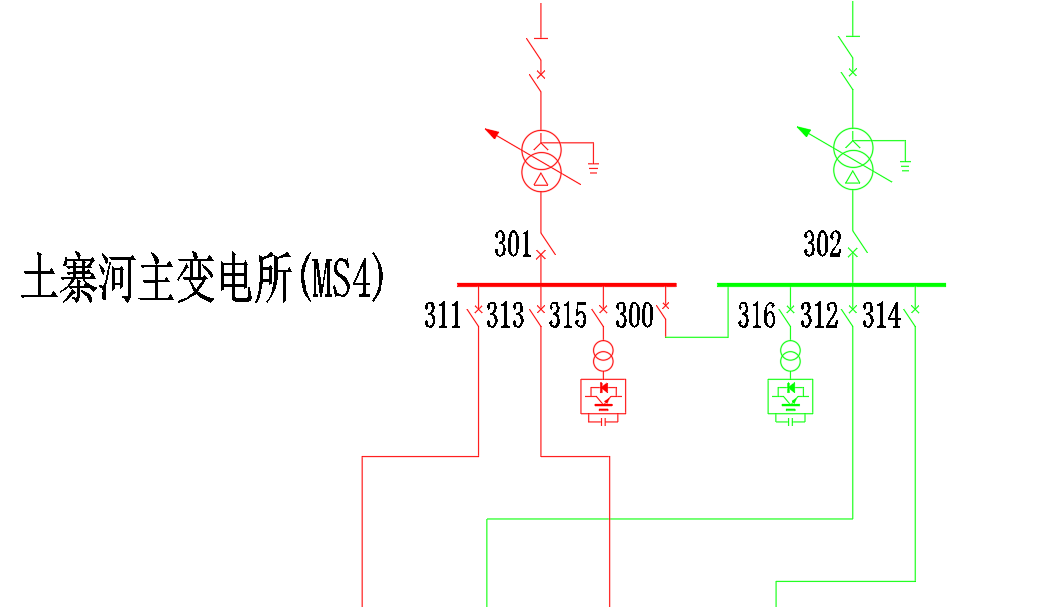
\includegraphics[width=0.5\textwidth]{土寨河主变电所.png}
	\caption{土寨河主变电所}
	\label{土寨河主变电所}
\end{figure}
\subsection{接线方式}
对于土寨河主变电所,其电力系统可以分为高压侧和中压侧两部分:

\begin{itemize}
	\item 高压侧:
	\begin{itemize}
		\item 土寨河主变电所的高压侧接线方式采用线路—变压器组接线方式。
	\end{itemize}
	\item 中压侧:
	\begin{itemize}
		\item 土寨河主变电所的中压侧采用$AC35kV$系统,以单母线分段形式运行,并配备母线分段开关。
		\item 主变电所的两个$AC35kV$进线电源分别引自$220kV/35kV$主变压器。
		\item 每段母线设置了3回$AC35kV$馈线,其中2回用于为下级各变电所提供$AC35kV$电源,而1回连接到动态无功补偿装置(SVG)。
		\item 每段母线还配置了一套动态无功补偿装置(SVG),这些SVG通过$AC35kV$断路器接入到母线上。
	\end{itemize}
\end{itemize}

这些配置和接线方式的设计用于确保土寨河主变电所的电力系统能够稳定运行,并提供所需的电源供应。
\subsection{运行方式}
\begin{enumerate}
	\item 高压侧:
	
	 
	在正常运行方式下,系统配置了两台主变压器,每台负责一路电源。如果主变压器的一、二级负荷负载较低,当系统出现故障时,恢复供电操作相对简单。只需将中压侧的负载转移到主变电所的另一路,使其承担全部一、二级负荷。然而,如果主变压器的一、二级负荷负载较高,系统发生故障时,需要通过与相邻主变电所的联络开关来转移部分负荷,以实现相互支援。
	
	当一台主变电所正在进行检修时,如果另一组线路变压器组的进线发生故障,整个主变电所将全部退出运行。在这种情况下,可以在两组进线之间连接一组带隔离开关的横跨条,以实现进线之间的相互支援。
	
	\item 中压侧: 
	
	
	在正常情况下,两段母线分别运行,牵引变电所和降压所可以从不同的母线段获取中压电源。如果主变电所的一段中压母线失电,另一段中压母线可以迅速恢复对牵引变电所和降压所的供电。
	
	
	当一段中压母线发生故障时,该母线上的进线开关将分闸,同时该段母线上的馈线连接的第一级牵引或降压变电所进线开关也会失压跳闸。与此同时,主变电所的另一段中压母线将继续供电。
\end{enumerate}
\section{跟随所主接线分析}
跟随所的接线图如图\ref{跟随所}所示:
\begin{figure}[h]
	\centering
	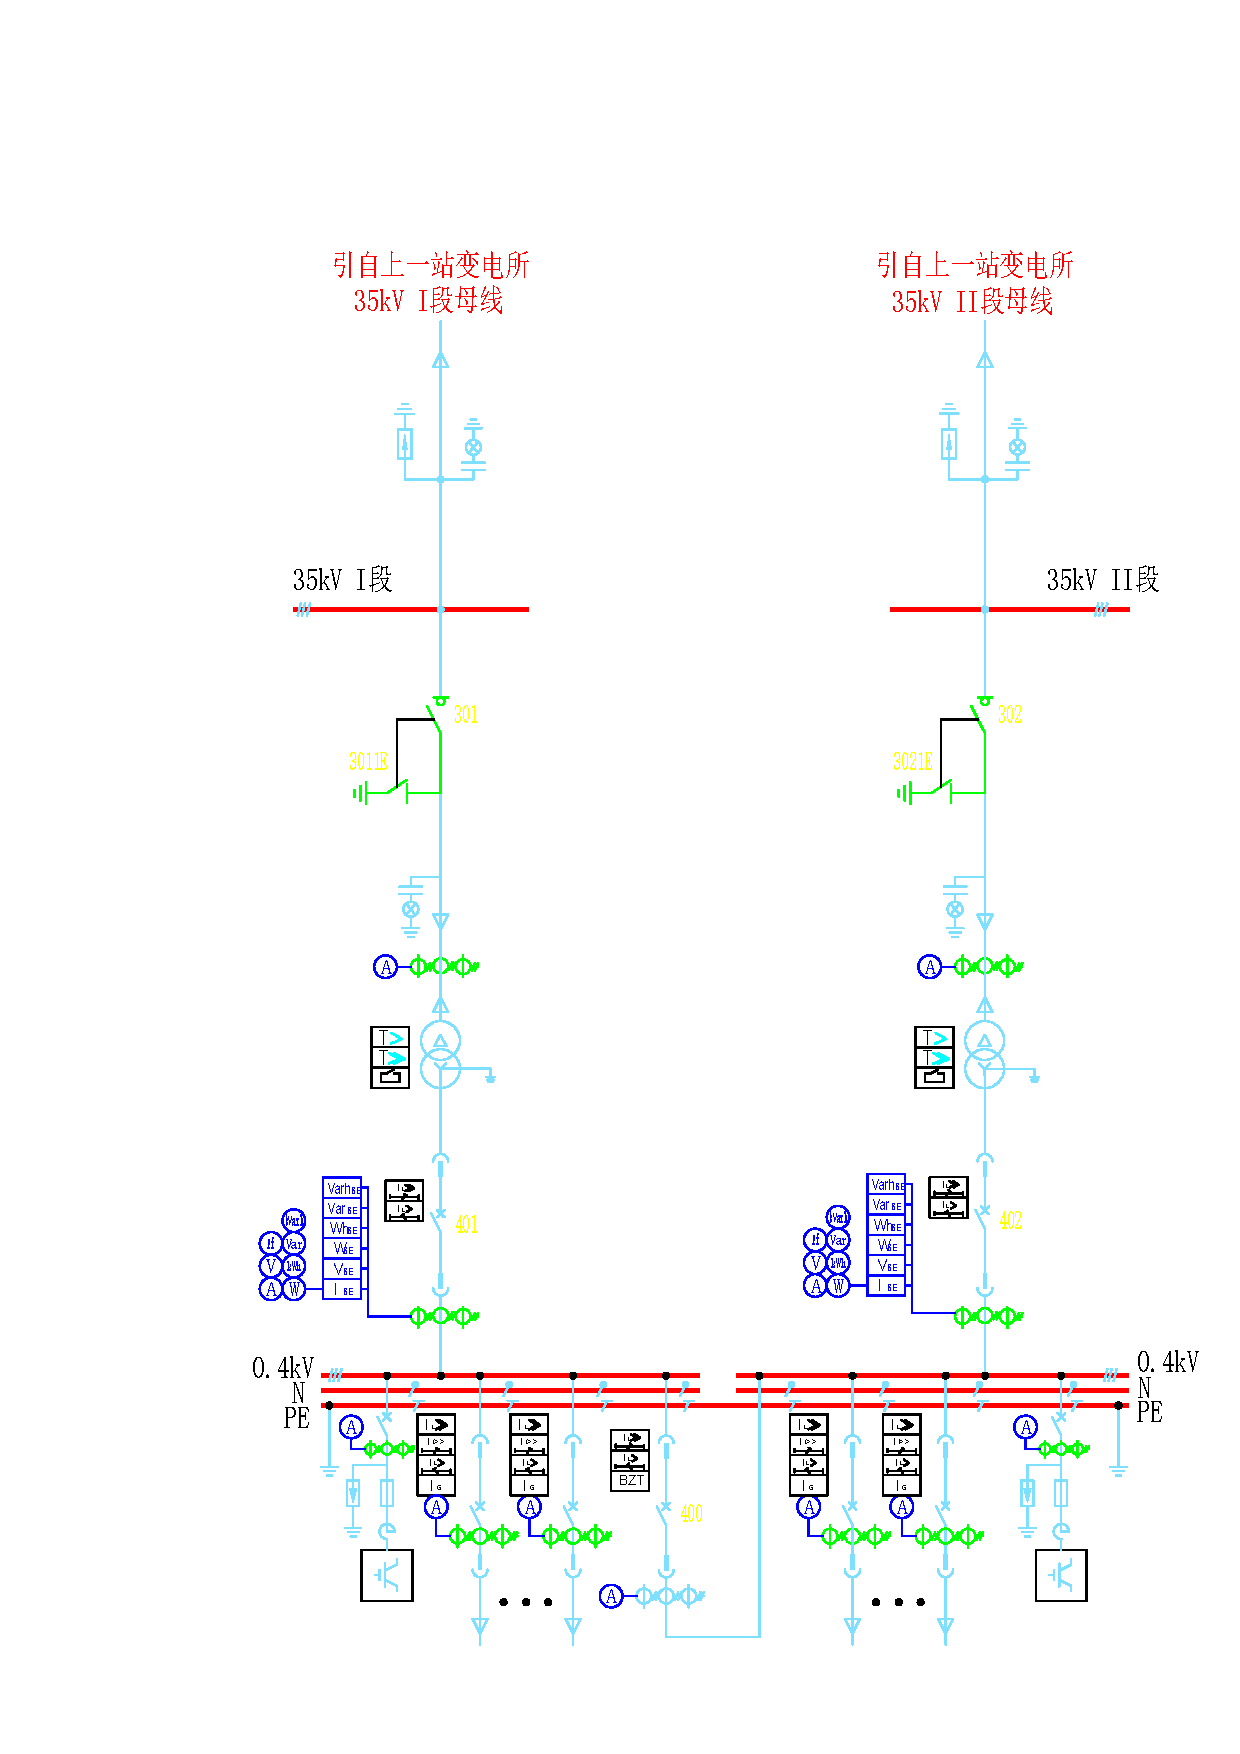
\includegraphics[width=0.5\textwidth]{跟随所.pdf}
	\caption{跟随所}
	\label{跟随所}
\end{figure}
\subsection{接线方式}
$AC35kV$侧采用线路变压器组接线,引入的两路$35kV$电源通过$35kV$负荷开关接到相应的两台配电变压器。两段$AC35kV$母线各设一组避雷器。

\subsection{运行方式}
在正常运行情况下,变电所两个$35kV$进线电源分别向所接的$35kV$母线的全部动力照明负荷提供电源。


当一路$AC35kV$进线电源失电时,该段电源所供的配电变压器退出运行,通过低压母线分段开关自动或手动合闸后,由另一个$35kV$进线电源向本所供电范围内的动力照明一、二级负荷供电。
\section{降压所主接线分析}
降压所的接线图如图\ref{降压所}所示:
\begin{figure}[h]
	\centering
	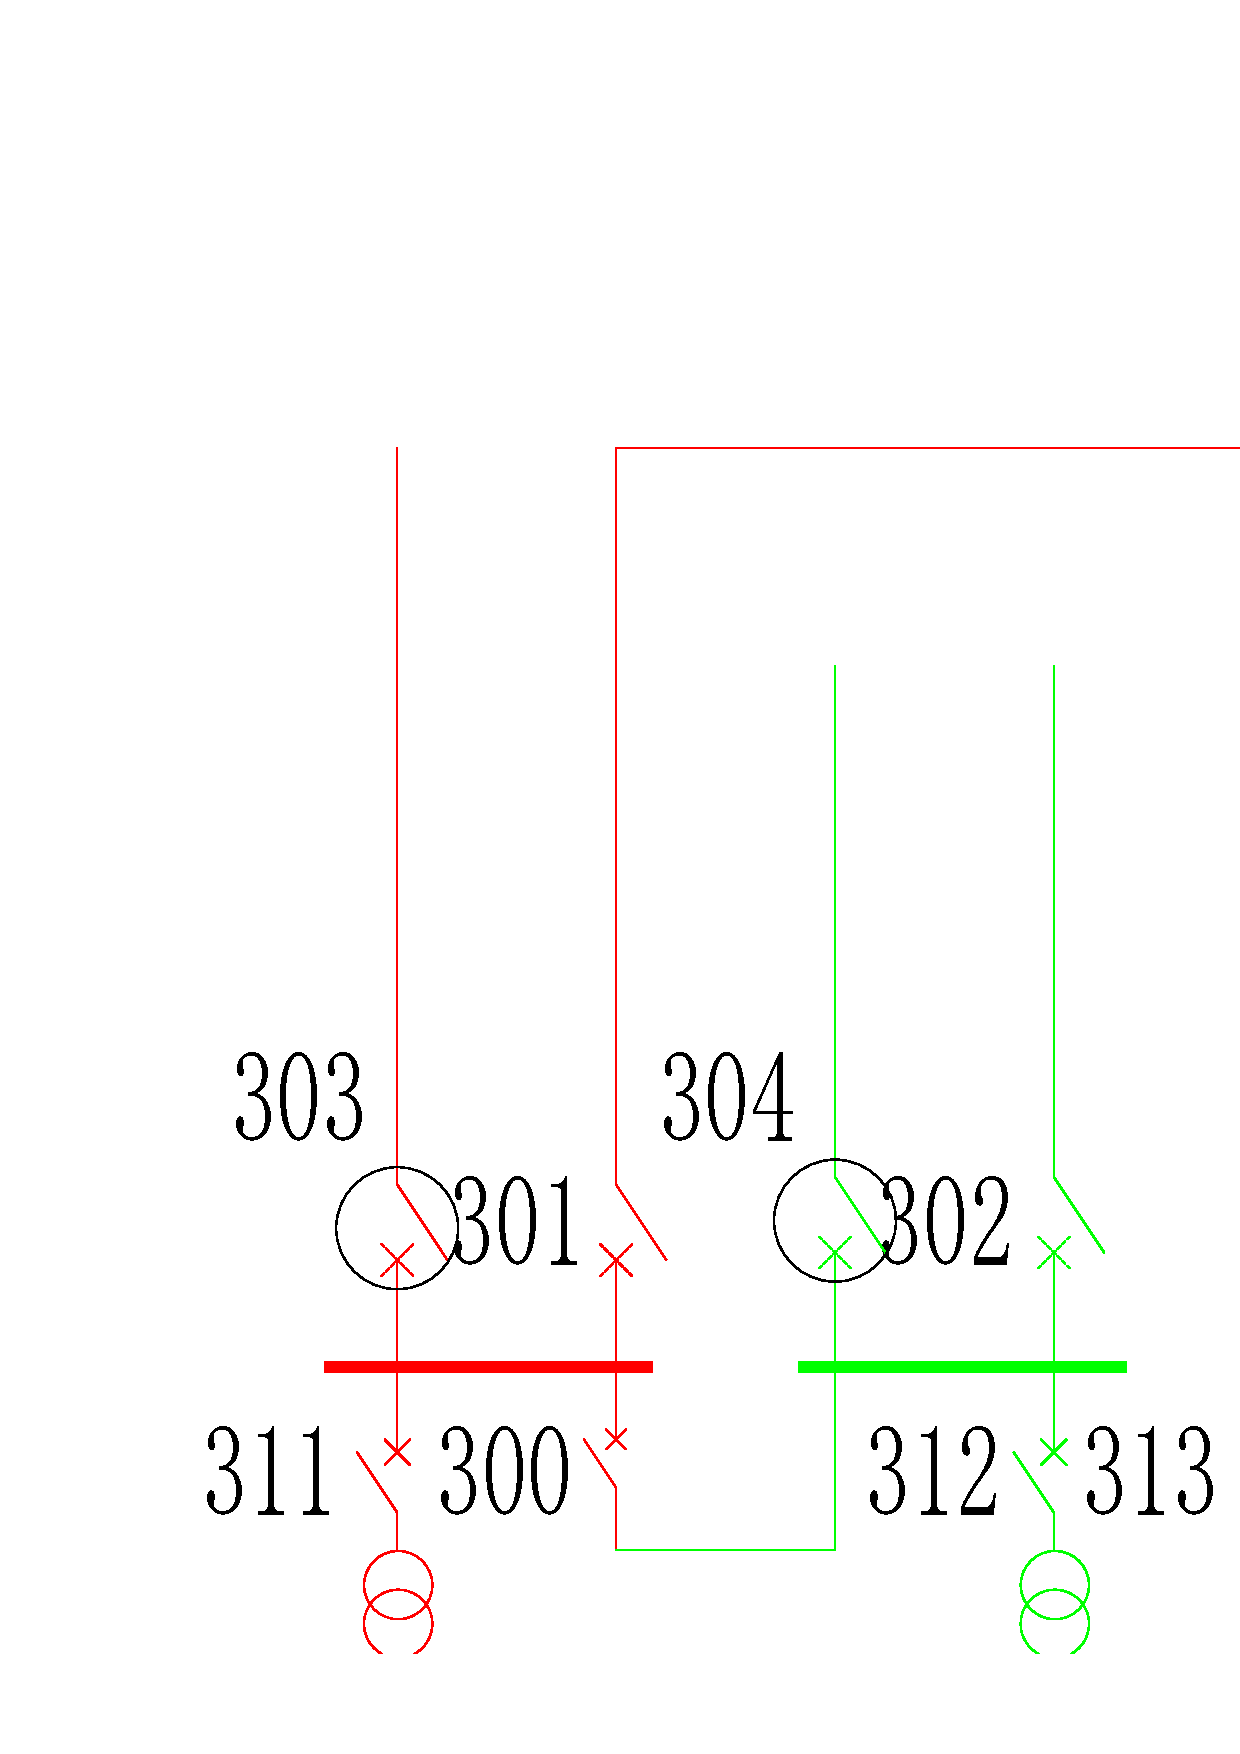
\includegraphics[width=0.5\textwidth]{降压所.pdf}
	\caption{降压所}
	\label{降压所}
\end{figure}
\subsection{接线方式}
$AC35kV$侧采用分段单母线接线,配备母线分段断路器。电力变电所的$1\#$进线电源引自上一站变电所的$Ⅰ$段母线,而$2\#$进线电源引自上一站变电所的$Ⅱ$段母线。此外,电力变电所配置了两台配电变压器,它们分别连接到两段$AC35kV$母线上。

\subsection{运行方式}
在正常运行情况下,两段母线分列运行,$AC35kV$母线分段开关处在分闸状态。两路进线电源分别为各自供电范围内的全部动力照明负荷提供电源。当一路$35kV$进线电源失电时,闭合$35kV$母线分段开关,由另一路$35kV$进线电源为该变电所供电范围内的动力照明负荷供电;此时另一路$35kV$进线电源再失电时,两路进线开关保持原状。

